\newpage
\subsection{Implementing empty}
\visHeader
\hypertarget{emptyPartition vis}{}

\begin{itemize}

\item[$\blacktriangleright$] Open a new activity diagram for \texttt{Partition.empty}. To begin building the \emph{for each} pattern, quick create a new story
node and edit its properties. Name it 'deleteCardsInPartition' and change the \texttt{Emph} from \texttt{StoryNode} to \texttt{ForEach}. You'll also want to
create the invoking partition object, so be sure to select that feature as well. As you can see, a \emph{for each} node is represented  as a stacked node to
indicate the potential for repetition.

\begin{figure}[htbp]
\begin{center}
  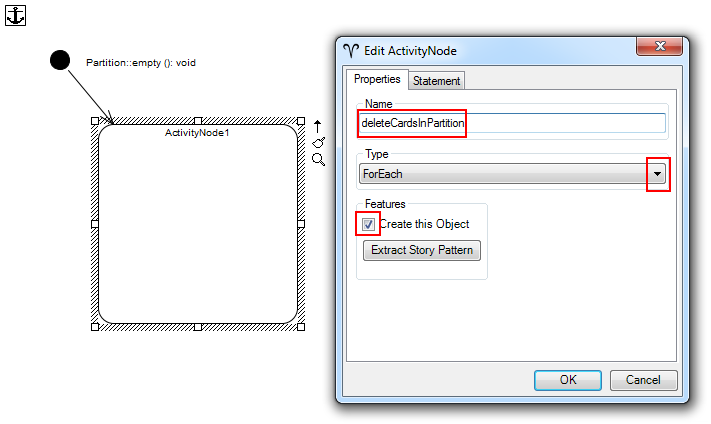
\includegraphics[width=0.9\textwidth]{ea_sdmEmptyNew}
  \caption{Creating a looping story node}  
  \label{fig:sdm_foreach}
\end{center}
\end{figure}

\item[$\blacktriangleright$] Now create the neccessary \texttt{card} variable needed to complete this SDM. Unlike \texttt{removeCard}\footnote{See
Fig.~\ref{fig:sdm_complete_control_flow}} however, the goal of \texttt{emptyCards} is not just to remove the link between the selected partition and card, we
want the matched \texttt{card} to be fully deleted. This means in the properties tab, after setting the name and binding state, you'll need to set the \emph{Binding
Operator} to \texttt{Destroy} (Fig.~\ref{fig:sdm_bindingOperator}).

\begin{figure}[htbp]
\begin{center}
  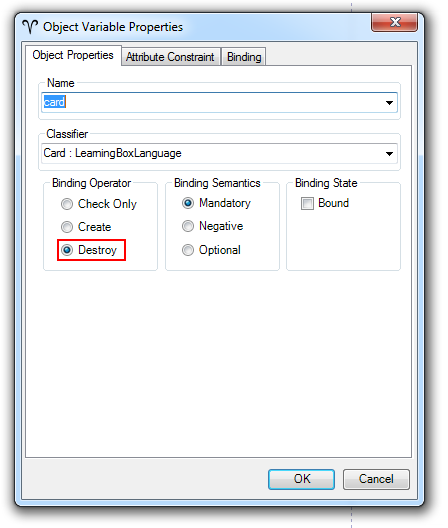
\includegraphics[width=0.65\textwidth]{ea_emptyBindingOperator}
  \caption{Editing \texttt{card} so the variable gets destroyed}  
  \label{fig:sdm_bindingOperator}
\end{center}
\end{figure}

\item[$\blacktriangleright$] Complete the story pattern as indicated in Fig.~\ref{fig:sdm_end}. Notice that the guard that terminates the looping node has an
\texttt{[end]} edge guard. Indeed, a \emph{for each} story node \emph{must} execute an \texttt{end} activity when all matches in the pattern have been
handled.

\begin{figure}[htbp]
\begin{center}
  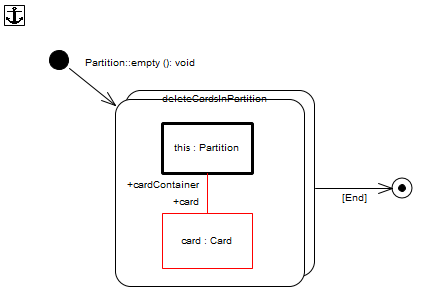
\includegraphics[width=0.8\textwidth]{ea_sdmEmptyComplete}
  \caption{Completed \texttt{empty} story pattern}  
  \label{fig:sdm_end}
\end{center}
\end{figure}

\item[$\blacktriangleright$] Done! You've now learned that in order to create a repeating action, all you need to do is change a standard standard story node
into a \texttt{for each} node, and include a edge guard. Inspect Figs. \ref{fig:emptyControlFlow} and \ref{fig:emptyPattern} to see how this is implemented
textually.

\fancyfoot[R]{ $\triangleright$ \hyperlink{sec:invertCard}{Next}} 

\end{itemize}

